\chapter{AHTR Modeling and Optimization Methodology}
In this chapter, I describe the modeling and optimization methodology of
\gls{ROLLO} \gls{AHTR} optimization for non-conventional geometries and parameters.
To wholly explore the design space enabled by additive manufacturing, the 
optimization tool should enable placement of fuel, moderation, and coolant material 
in any possible location, within physical limits. 
Since exploration of non-conventional geometries and parameters has barely been
attempted (previous attempts described in Section \ref{sec:lit-review-reactor-arbitrary}), 
this dissertation attempts a first go at beginning to explore the large design space.  
The work done for this dissertation is only an intermediate step towards developing 
a truly arbitrary geometry expression. 

%In the subsequent sections, I will define the optimization problem, describe the 
%AHTR geometries . 
%Then, I will describe the software used to model them and the specific models. 

\section{Optimization Problem Definition}
\label{sec:opt-problem}
In an effort towards optimizing reactor design for non-conventional geometries 
and parameters.
I chose to vary the following \gls{AHTR} parameters: 
\begin{itemize}
    \item \gls{TRISO} particle packing fraction distribution, 
    $\rho_{TRISO}(\vec{r})$
    \item Total fuel packing fraction
    \item \gls{FLiBe} coolant channel shape 
\end{itemize} 
The TRISO packing fraction distribution variation enables exploration of how 
heterogenous fuel distributions impact reactor performance.
In Chapter \ref{chap:fhr-benchmark}, the results demonstrated that increased fuel 
packing does not always correspond with increased $k_{eff}$ due to self-shielding
effects. 
Varying total fuel packing fraction and TRISO distribution synergistically enables exploration of
how heterogenous TRISO distribution could minimize self-shielding and in turn reduce the fuel 
required for a reactor design. 
The FliBe coolant channel shape variation enables exploration of how non-uniform 
channel shapes impact reactor performance. 

I selected three key \gls{AHTR} optimization objectives that address contrasting reactor 
core qualities. 
Table \ref{tab:objectives} describes each objective, how I quantified them, and the motivation.
\begin{table}[]
    \centering
    \onehalfspacing
    \caption{\acrfull{ROLLO} optimization problem objectives with their quantification 
    descriptions, and motivation.}
	\label{tab:objectives}
    \footnotesize
    \begin{tabular}{p{4cm}p{5cm}p{5cm}}
    \hline 
    \textbf{Objective}& \textbf{Quantification}& \textbf{Motivation} \\
    \hline
    Minimize fuel amount & Minimize total fuel packing fraction & Cost savings, Non-proliferation \\ 
    \hline
    Maximize heat transfer & Minimize maximum temperature & Enable system to perform at a higher power with minimized thermal stress \\
    \hline
    Minimize power peaking & Minimize power peaking factor normalized by fuel distribution & Efficient fuel utilization, longer core life, safety\\
    \hline
    \end{tabular}
\end{table}
I will vary the described parameters in the \gls{AHTR} plank and \gls{AHTR} one-third assembly 
geometries to optimize the described objectives. 
The plank optimization acts as a preliminary study to inform the more complex \gls{AHTR} one-third
assembly optimization setup. 
In the next section, I will describe both geometries. 

\section{AHTR Geometry for Optimization Problem}
The optimization process is applied to both the \gls{AHTR} plank and \gls{AHTR} one-third
assembly geometries.
The geometries are adapted from the \gls{AHTR} design in the \gls{FHR} benchmark,
outlined in Chapter \ref{chap:fhr-benchmark}.
The main differences occur in the fuel plank region (see Figure \ref{fig:ahtr-fuel-assembly}). 
In the \gls{FHR} benchmark, the TRISO particles are arranged in rectangular lattices within
two fuel stripes in the plank. 
For the optimization problem, I instead discretized each plank into ten cells with random 
TRISO packing and an individually controlled packing fraction. 
I also omit the graphite spacers. 

\subsection{AHTR Plank Geometry}
\label{sec:ahtr-plank-geometry}
The \gls{AHTR} plank is a single graphite fuel plank model from the \gls{AHTR} design (Figure 
\ref{fig:ahtr-fuel-assembly}). 
I modified the fuel plank to be straightened with perpendicular sides, instead 
of slanted as in Figure \ref{fig:ahtr-fuel-plank}, for ease of modeling. 
The original slanted \gls{AHTR} geometry will be used for the complex one-third assembly 
optimization setup. 
Figure \ref{fig:straightened_plank} illustrates the straightened fuel plank with 
ten fuel cells with random \gls{TRISO} packing.
\begin{figure}[]
    \centering
    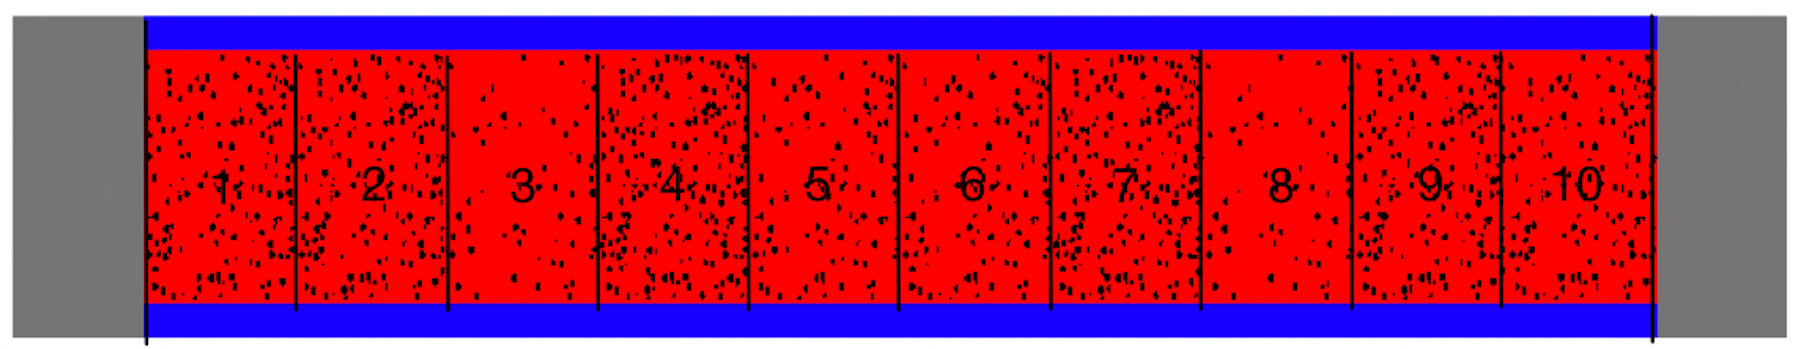
\includegraphics[width=0.85\linewidth]{straightened_plank.png}
    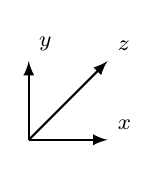
\begin{tikzpicture}
        \draw[ thick,-latex] (0,0) -- (1,0) node[anchor=south west] {$x$};
        \draw[ thick,-latex] (0,0) -- (0,1) node[anchor=south west] {$y$};
        \draw[ thick,-latex] (0,0) -- (1,1) node[anchor=south west] {$z$};
       \tkzText[above](-0.3,-0.7){}
       \end{tikzpicture} 
    \raggedright
    \resizebox{0.3\textwidth}{!}{
        \hspace{1cm}
        \fbox{\begin{tabular}{ll}
            \textcolor{fhrblue}{$\blacksquare$} & FLiBe \\
            \textcolor{fhrgrey}{$\blacksquare$} & Graphite (Structure)\\
            \textcolor{fhrred}{$\blacksquare$} & Graphite (Fuel Plank) \\
            \textcolor{fhrblack}{$\blacksquare$} & TRISO particle 

            \end{tabular}}}
    \caption{Straightened \acrfull{AHTR} fuel plank with 10 fuel cells with random 
    TRISO packing. Original slanted fuel planks can be seen in Figures 
    \ref{fig:ahtr-fuel-assembly} and \ref{fig:ahtr-fuel-plank}.}
    \label{fig:straightened_plank}
\end{figure}
The plank has $27.1 \times 3.25 \times 1.85\ cm^3$ dimensions with reflective 
boundary conditions.

I used the same materials as in the \gls{FHR} benchmark (Chapter \ref{chap:fhr-benchmark}), 
except that I homogenized each \gls{TRISO} particle's four outer layers: 
porous carbon buffer, inner pyrolytic carbon, silicon carbide layer, and the 
outer pyrolytic carbon. 
The \gls{TRISO} particle dimensions remain the same.
Table \ref{tab:keff_triso} reports OpenMC's reported $k_{eff}$ for this original 
straightened \gls{AHTR} configuration with and without the outer layer \gls{TRISO} 
homogenization.
\begin{table}[]
    \centering
    \onehalfspacing
    \caption{Straightened \acrfull{AHTR} fuel plank $k_{eff}$ for case with 
    no \gls{TRISO} homogenization and case with homogenization of the four outer 
    layers. Both simulations were run on one BlueWaters XE Node.}
	\label{tab:keff_triso}
    \footnotesize
    \begin{tabular}{llc}
    \hline 
    \textbf{TRISO Homogenization}& \textbf{$k_{eff}$} & \textbf{Simulation time [s]}  \\
    \hline 
    None & $1.38548 \pm 0.00124$ & 233\\ 
    Four outer layers & $1.38625 \pm 0.00109$ & 168\\ 
    \hline
    \end{tabular}
\end{table}
The \gls{TRISO} particle outer four-layer homogenization resulted in a $30\%$ 
speed-up without compromising accuracy with $k_{eff}$ values within each 
other's uncertainty.

% coolant channel shape variation

\subsection{AHTR One-Third Assembly Geometry}
The \gls{AHTR} one-third assembly is one-diamond shape sector of the \gls{AHTR} assembly and
contains six fuel planks.
Each graphite plank has graphite buffers and ten rectangular prism fuel cells 
with random TRISO packing and individually controlled packing fraction. 
Figure \ref{fig:ahtr_assembly} shows the one-third \gls{AHTR} assembly with 10 x 6 fuel cells with 
random \gls{TRISO} packing.
\begin{figure}[]
    \centering
    \begin{subfigure}{.7\textwidth}
    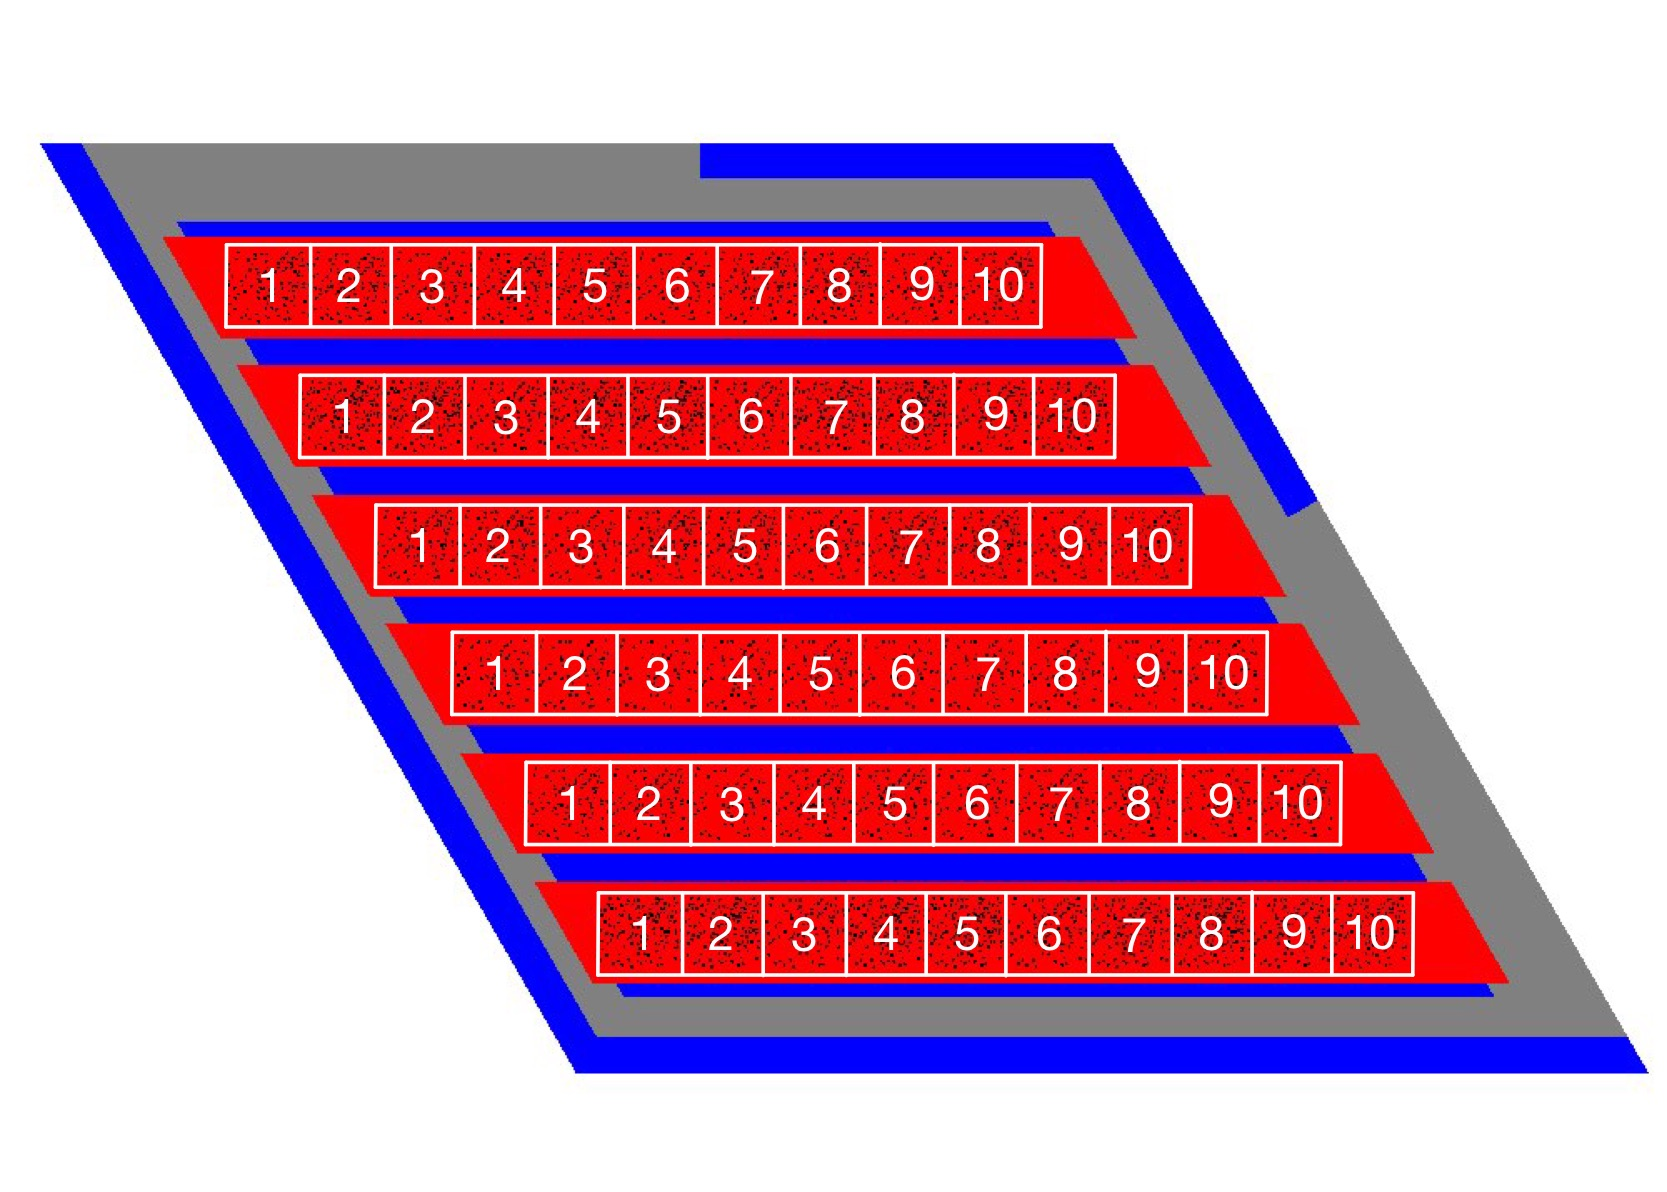
\includegraphics[width=\linewidth]{ahtr_assembly.png}
    \end{subfigure}%
    \begin{subfigure}{.3\textwidth}
        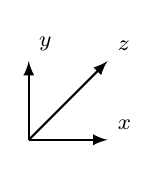
\begin{tikzpicture}
            \draw[ thick,-latex] (0,0) -- (1,0) node[anchor=south west] {$x$};
            \draw[ thick,-latex] (0,0) -- (0,1) node[anchor=south west] {$y$};
            \draw[ thick,-latex] (0,0) -- (1,1) node[anchor=south west] {$z$};
           \tkzText[above](-0.3,-0.7){}
        \end{tikzpicture} 
        \vspace{1cm}
        \fbox{\begin{tabular}{ll}
            \textcolor{fhrblue}{$\blacksquare$} & FLiBe \\
            \textcolor{fhrgrey}{$\blacksquare$} & Graphite (Structure)\\
            \textcolor{fhrred}{$\blacksquare$} & Graphite (Fuel Plank) \\
            \textcolor{fhrblack}{$\blacksquare$} & TRISO particle 
            \end{tabular}}
    \end{subfigure}
    \caption{\gls{AHTR} assembly with 10 fuel cells in each graphite plank with random 
    TRISO packing. Original \gls{FHR} benchmark fuel assembly with fuel stripes can be seen in 
    Figure \ref{fig:ahtr-fuel-assembly}.}
    \label{fig:ahtr_assembly}
\end{figure}
The assembly model also uses the \gls{TRISO} particle outer four layer homogenization described 
in Section \ref{sec:ahtr-plank-geometry}.

% coolant channel shape variation

\section{AHTR Model Workflow}
\gls{ROLLO} drives the evolutionary algorithm optimization process. 
In the \gls{ROLLO} input file, I will define control variables for the genetic algorithm 
to vary. 
These control variables are values used to control the \gls{AHTR} parameters described in 
Section \ref{sec:opt-problem}.
These control variables will be input into templated nuclear software to model different 
AHTR geometries.
The software will then run the \gls{AHTR} models and calculate the optimization objective 
and constraint values. 

In this work, I use OpenMC \cite{romano_openmc:_2015} to model \gls{AHTR}'s neutronics 
and Moltres \cite{lindsay_introduction_2018} to model the \gls{AHTR}'s multi-physics. 
OpenMC is an open-source Monte Carlo neutron transport code capable of 
performing k-eigenvalue calculations on models built using either constructive 
solid geometry or CAD representation. 
Moltres is an open-source tool designed to simulate \glspl{MSR} using 
deterministic neutronics and thermal-hydraulics implemented as an application 
atop the \gls{MOOSE} finite-element framework.  
Moltres solves arbitrary-group neutron diffusion, temperature, and precursor 
governing equations on a single mesh and can be deployed on an arbitrary number 
of processing units \cite{lindsay_introduction_2018}.
OpenMC and Moltres are both open-source, well-documented, well-supported, and 
Github version-controlled codes that can run in parallel on \gls{HPC} machines.

In this section, I describe the \gls{AHTR} modeling workflow: from the AHTR geometry 
variation input parameters, to the OpenMC and Moltres models, and finally the 
output and constraint values. 
This corresponds to the \textit{evaluate population} orange blocks in Figure 
\ref{fig:genetic_alg_nuclear}'s genetic algorithm flow chart.
Figure \ref{fig:ahtr-model-flow} illustrates the modeling workflow. 
\begin{figure}[]
    \centering
    \begin{tikzpicture}[node distance=0.5cm]
        \tikzstyle{every node}=[font=\footnotesize]
        \node (1) [e72block] {\textit{Total PF}};
        \node (2) [b72block, right=of 1] {PF};
        \node (3) [e72block, above=of 2] {Input Parameters};
        \node (4) [e72block, below=of 1] {$\rho_{TRISO}(\vec{r})$};
        \node (5) [b72block, right=of 4] {a, b, c, d, e, f};
        \node (6) [e72block, below=of 4] {FliBE Coolant Channel Shape};
        \node (7) [b72block, right=of 6] {$r_{top}$, $r_{bot}$};
        \node (8) [o72block, right=of 2, xshift=0.8cm, yshift=0.5cm] {OpenMC Model};
        \node (9) [e72block, above=of 8] {Input Files};
        \node (10) [o72block, right=of 5, xshift=0.8cm] {Group Constants};
        \node (11) [o72block, right=of 7, xshift=0.8cm, yshift=-0.5cm] {Moltres Model};
        \node (12) [b72block, right=of 8, xshift=0.8cm, yshift=0.8cm] {$k_{eff}$}; 
        \node (13) [e72block, above=of 12] {Constraints};
        \node (14) [e72block, below=of 12] {Objectives};
        \node (15) [b72block, below=of 14] {PF};
        \node (16) [b72block, below=of 15] {PPF};
        \node (17) [b72block, below=of 16] {$T_{max}$};
        \draw [arrow] (2) -- ([shift={(0cm,0cm)}]2.east) -- ([shift={(0cm,0cm)}]8.west);
        \draw [arrow] (5) -- ([shift={(0cm,0cm)}]5.east) -- ([shift={(0cm,0cm)}]8.west);
        \draw [arrow] (7) -- ([shift={(0cm,0cm)}]7.east) -- ([shift={(0cm,0cm)}]8.west);
        \draw [arrow] (7) -- ([shift={(0cm,0cm)}]7.east) -- ([shift={(0cm,0cm)}]11.west);
        \draw [arrow] (8) -- ([shift={(0cm,0cm)}]8.south) -- node[anchor=west] {generates} ([shift={(0cm,0cm)}]10.north);
        \draw [arrow] (10) -- ([shift={(0cm,0cm)}]10.south) -- node[anchor=west] {input into} ([shift={(0cm,0cm)}]11.north);
        \draw [arrow] (8) -- ([shift={(0cm,0cm)}]8.east) -- ([shift={(0cm,0cm)}]12.west);
        \draw [arrow] (8) -- ([shift={(0cm,0cm)}]8.east) -- ([shift={(0cm,0cm)}]15.west);
        \draw [arrow] (8) -- ([shift={(0cm,0cm)}]8.east) -- ([shift={(0cm,0cm)}]16.west);
        \draw [arrow] (11) -- ([shift={(0cm,0cm)}]11.east) -- ([shift={(0cm,0cm)}]17.west);
    \end{tikzpicture}
    \caption{\acrfull{AHTR} modeling workflow in ROLLO optimization.} 
    \label{fig:ahtr-model-flow}
\end{figure}

\subsection{Input Parameter Modeling}
In this section, I describe how I modeled the \gls{AHTR} parameter variations: total fuel packing 
fraction, \gls{TRISO} particle packing fraction distribution, and \gls{FLiBe} coolant channel shape. 
For both the \gls{AHTR} plank and one-third assembly models, total fuel packing fraction parameter 
is a single numerical input.
I describe the other two parameters for both the \gls{AHTR} plank and one-third assembly. 

\subsubsection{Input Parameter Modeling: TRISO particle packing fraction distribution}
For both the \gls{AHTR} plank and one-third assembly, I utilize sine distributions to govern the 
\gls{TRISO} particle packing fraction distribution. 
Based on the sine distributions, the model calculates the packing fraction in each fuel cell, then use 
OpenMC's \texttt{pack\_spheres} function to randomly disperse the calculated packing fraction in each 
fuel cell. 
For the \gls{AHTR} plank, one sine distribution governs the \gls{TRISO} packing fraction distribution 
across the fuel plank's x-direction. 
For the \gls{AHTR} one-third assembly, two sine distributions govern the \gls{TRISO} packing fraction 
distribution across each fuel plank's x-direction, and the assembly's y-direction, respectively. 

For the \gls{AHTR} plank, a sine distribution governs the \gls{TRISO} particle packing fraction 
distribution across the ten fuel cells, illustrated in Figure \ref{fig:straightened_plank}:
\begin{align}
    PF(x) &= \left(a\cdot sin(b\cdot x + c) + 2\right) \cdot NF\\
    \intertext{where}
    PF &= \mbox{packing fraction } [-] \nonumber \\ 
    a &= \mbox{amplitude, peak deviation of the function from zero } [-] \nonumber \\
    b &= \mbox{angular frequency, rate of change of the function argument } [\frac{radians}{cm}] \nonumber \\
    c &= \mbox{phase, the position in its cycle the oscillation is at t = 0 } [radians]\nonumber \\
    x &= \mbox{midpoint value for each cell } [cm]\nonumber \\
    NF &= \mbox{normalization factor } [-]\nonumber
\end{align}
The sine distribution's coefficients, \textit{a b c}, are the control variables \gls{ROLLO} 
utilizes to control the TRISO packing fraction distribution in the plank.
Thus, \gls{ROLLO} will vary $a, b, c$ constants to find an optimal TRISO particle 
sine distribution. 
The normalization factor ensures the correct total packing fraction 
in the plank regardless the \gls{TRISO} particle distribution.

For example in a \gls{AHTR} plank with a 0.0979 total packing fraction, and packing fraction 
distribution of $PF(x) = \left(0.5\cdot sin(\frac{\pi}{3}\cdot x + \pi) + 2\right)  \cdot NF$, 
results in the following packing fractions for the ten cells: 0.103, 0.120, 
0.049, 0.138, 0.076, 0.081, 0.136, 0.048, 0.125, and 0.098. 
Figure \ref{fig:triso_distribution} shows this sine distribution, highlights 
the packing fraction at the respective midpoints, and displays the plank's x-y 
axis view with packing fraction varying based on this sine distribution. 
\begin{figure}[]
    \centering
    \makebox[\textwidth][c]{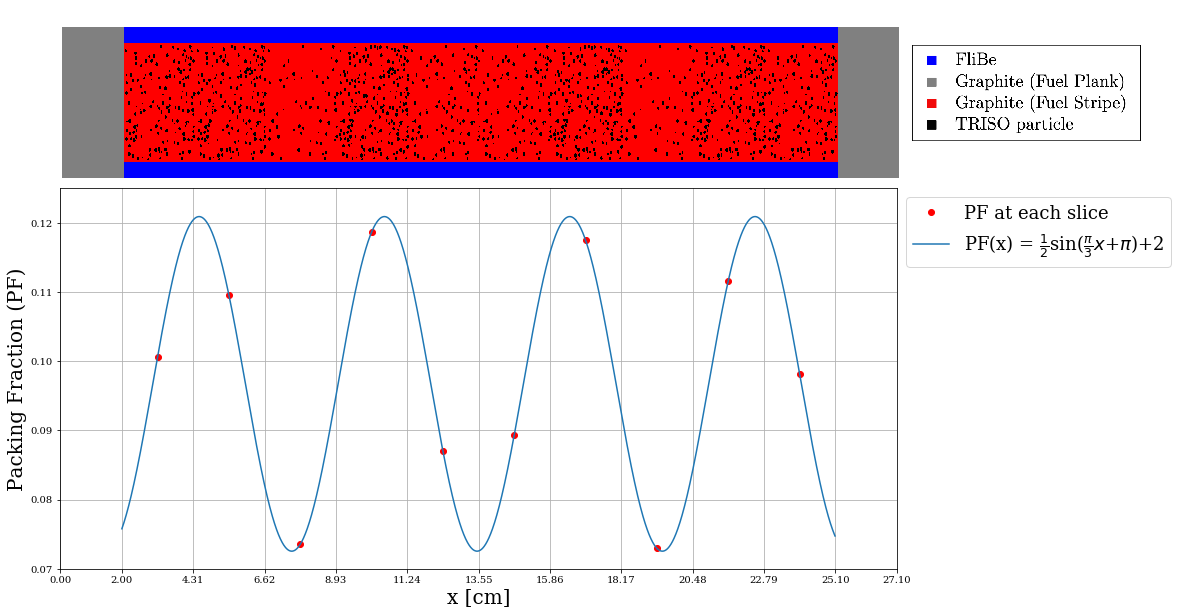
\includegraphics[width=1.1\linewidth]{triso_distribution_sine.png}} 
    \caption{Above: Straightened \acrfull{AHTR} fuel plank with varying \gls{TRISO} particle 
    distribution across ten cells based on the sine distribution. 
    Below: $PF(x) = (0.5\ sin(\frac{\pi}{3}x + \pi) + 2)  \times NF$ 
    sine distribution with red points indicating the packing fraction at each cell. }
    \label{fig:triso_distribution}
\end{figure}

For the \gls{AHTR} one-third assembly, two sine distributions govern the x and y direction
\gls{TRISO} particle packing fraction distributions in the 10 x 6 fuel cell shape, illustrated in 
Figure \ref{fig:ahtr_assembly}:
\begin{align}
    PF(x, y) &= \left(a\cdot sin(b\cdot x + c) + 2\right) 
    \cdot \left(d\cdot sin(e\cdot y + f) + 2\right) \cdot NF \\
    \intertext{where}
    PF &= \mbox{packing fraction } [-] \nonumber \\ 
    a, d &= \mbox{amplitude, peak deviation of the function from zero } [-] \nonumber \\
    b, e &= \mbox{angular frequency, rate of change of the function argument } [\frac{radians}{cm}] \nonumber \\
    c, f &= \mbox{phase, the position in its cycle the oscillation is at t = 0 } [radians]\nonumber \\
    x &= \mbox{midpoint value for each x-direction fuel cell } [cm]\nonumber \\
    y &= \mbox{midpoint value for fuel plank } [cm]\nonumber \\
    NF &= \mbox{normalization factor } [-]\nonumber
\end{align}
The sine distribution's coefficients, \textit{a b c d e f}, are the control variables \gls{ROLLO} 
utilizes to control the TRISO packing fraction distribution in the assembly.
Thus, \gls{ROLLO} will vary \textit{a b c d e f} constants to find an optimal TRISO particle 
distribution. 
The normalization factor ensures the correct total packing fraction 
in the plank regardless the \gls{TRISO} particle distribution.

For example in an \gls{AHTR} one-third assembly with a 0.1 total packing fraction, and packing 
fraction distribution of $PF(x, y) = \left(0.5\cdot sin(1\cdot x + 1) + 2\right) \cdot 
\left(0.7\cdot sin(1.5\cdot y + 2) + 2\right) \cdot NF$ results in the packing fraction 
distribution shown in Figure \ref{fig:ahtr-assem-triso-distr-squares}.
This corresponds to the one-third assembly with varying TRISO distribution in its fuel 
cells, shown in Figure \ref{fig:ahtr-assem-triso-distr}. 
\begin{figure}[]
    \centering
    \begin{subfigure}{0.49\textwidth}
        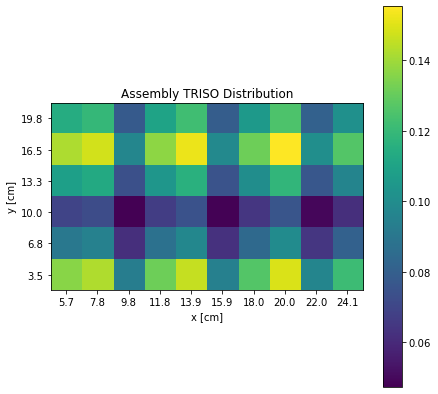
\includegraphics[width=\linewidth]{ahtr-assem-triso-distr-squares.png}
        \caption{}
        \label{fig:ahtr-assem-triso-distr-squares} 
    \end{subfigure}
    \begin{subfigure}{0.49\textwidth}
        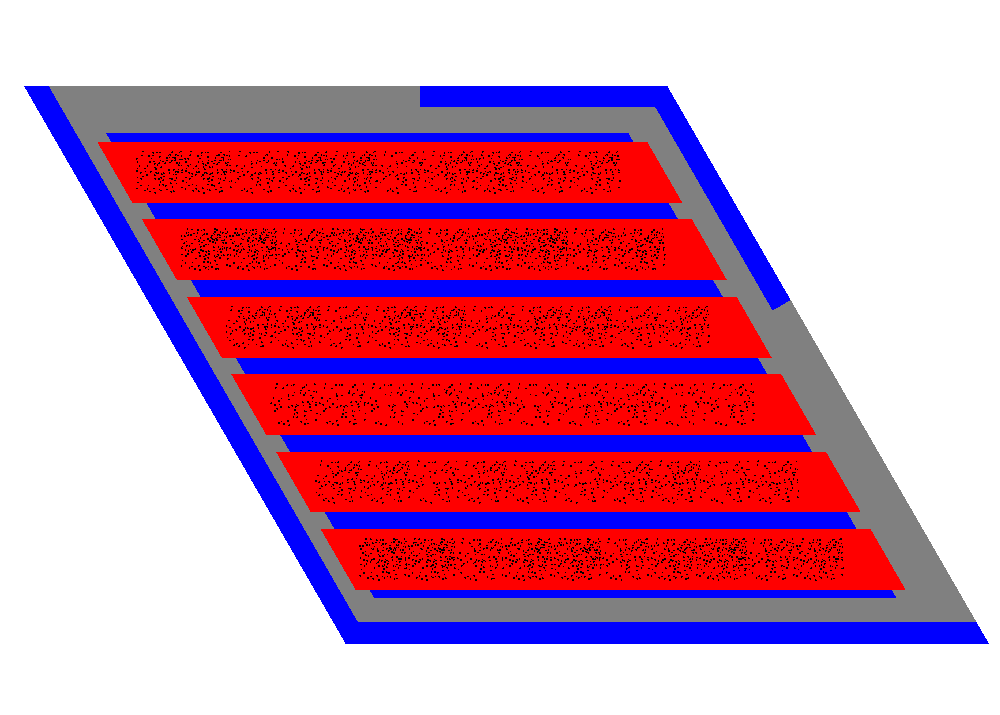
\includegraphics[width=\linewidth]{ahtr-assem-triso-distr.png}
        \raggedleft
        \resizebox{0.5\textwidth}{!}{
        \hspace{1cm}
        \fbox{\begin{tabular}{ll}
            \textcolor{fhrblue}{$\blacksquare$} & FLiBe \\
            \textcolor{fhrgrey}{$\blacksquare$} & Graphite (Structure) \\
            \textcolor{fhrred}{$\blacksquare$} & Graphite (Fuel Plank) \\
            \textcolor{fhrblack}{$\blacksquare$} & TRISO particle 
        \end{tabular}}}
        \caption{}
        \label{fig:ahtr-assem-triso-distr} 
    \end{subfigure}
    \caption{}
\end{figure}

\subsubsection{Input Parameter Modeling: FliBe Coolant Channel Shape}
I model the variation in coolant channel shape with a sinusoidal-like pattern.
I use cylinder surfaces in OpenMC, instead of a sinusoidal function. 
Creating complicated sinusoidal shapes in OpenMC requires the use of DAGMC, a CAD based tool, 
which is out of scope of the dissertation.
By varying the radius of the cylinder, the depth and frequency of the coolant channel shape 
minimics a sinusoidal-like pattern.
I vary the FliBE coolant channel shape while holding the total coolant area constant. 

For the \gls{AHTR} plank, $radius_{top}$ and $radius_{bot}$ variables control the coolant channel 
shape on the bottom and top FliBe channels. 
Figure \ref{fig:coolant-channel-shape} shows the \gls{AHTR} plank's coolant channel shape 
for $radius_{top} = 0.2$ and $radius_{bot} = 0.3$.
\begin{figure}[]
    \centering
        
\includegraphics[width=\linewidth]{coolant-channel-shape.png}
    \raggedright
    \resizebox{0.3\textwidth}{!}{
        \hspace{1cm}
        \fbox{\begin{tabular}{ll}
            \textcolor{fhrblue}{$\blacksquare$} & FLiBe Coolant\\
            \textcolor{fhrgrey}{$\blacksquare$} & Graphite (Structure) \\
            \textcolor{fhrred}{$\blacksquare$} & Graphite (Fuel Plank) \\
            \textcolor{fhrblack}{$\blacksquare$} & TRISO particle 
        \end{tabular}}}
    \caption{AHTR Fuel Plank with Coolant Shape Variation, $radius_{top} 
    = 0.2$ and $radius_{bot} = 0.3$.}  
    \label{fig:coolant-channel-shape}
\end{figure}
$radius_{top}$ and $radius_{bot}$ are the control variables \gls{ROLLO} 
utilizes to control the coolant channel shape in the \gls{AHTR} plank.
Thus, \gls{ROLLO} will vary $radius_{top}$ and $radius_{bot}$ to find an optimal coolant 
channel shape.

% Assembly COolant channel shape variation

\subsection{AHTR OpenMC and Moltres Models}
\label{sec:ahtr-moltres-hom}
The input parameter modeling outlined in the previous section are inputs into 
the OpenMC neutronics model. 
The total packing fraction, TRISO particle distribution, and FliBE coolant 
channel shape are reflected in the OpenMC input file. 
Thus, there is TRISO level fidelity in the OpenMC neutronics model. 
The OpenMC neutronics model outputs the $k_{eff}$ constraint value, and the 
total packing fraction, and normalized power peaking factor output values. 
Section \ref{sec:ahtr_slab_output} gives further description of calculation for 
each output and constraint parameter.

For the Moltres model, a TRISO-level fidelity mesh file is impractical 
and will result in an extremely long Moltres runtimes. 
Moltres accepts group constant data from OpenMC for the Moltres multigroup 
neutron diffusion calculations and a mesh file representing the reactor geometry. 
Thus, for a successful \gls{AHTR} Moltres simulation, I established 
suitable spatial and energy homogenization that preserves accuracy while 
maintaining an acceptable runtime.
For both the \gls{AHTR} plank and one-third assembly models, I used the four group 
energy structure derived by Gentry et al. \cite{gentry_development_2016} for \gls{AHTR} 
geometries. 
Table \ref{tab:energy_structures} defines the group boundaries. 
\begin{table}[]
    \centering
    \onehalfspacing
    \caption{4-group energy structures for \acrfull{AHTR} geometry 
    derived by \cite{gentry_development_2016}.}
	\label{tab:energy_structures}
    \footnotesize
    \begin{tabular}{lll}
    \hline
    \multicolumn{3}{c}{\textbf{Group Boundaries [MeV]}} \\ 
    \hline
    \textbf{Group $\#$}& \textbf{Upper Bound} & \textbf{Lower Bound}  \\
    \hline 
    1 & $2.0000\times 10^1$ & $9.1188\times 10^{-3}$ \\ 
    2 & $9.1188\times 10^{-3}$ & $2.9023\times 10^{-5}$\\
    3 & $2.9023\times 10^{-5}$ & $1.8554\times 10^{-6}$\\
    4 & $1.8554\times 10^{-6}$ & $1.0000\times 10^{-12}$\\
    \hline
    \end{tabular}
\end{table}

For spatial homogenization of the straightened \gls{AHTR} fuel plank, I used 
OpenMC's \textit{cell} domain type to compute multigroup cross sections for 
different \textit{cells}. 
I discretized the plank into 13 \textit{cells}: FLiBe, left graphite, right 
graphite, and ten fuel cells (each cell has a different packing fraction). 
Figure \ref{fig:straightened_slab_mg} illustrates the \gls{AHTR} spatial 
homogenization for the OpenMC multigroup calculation. 
\begin{figure}[]
    \centering
    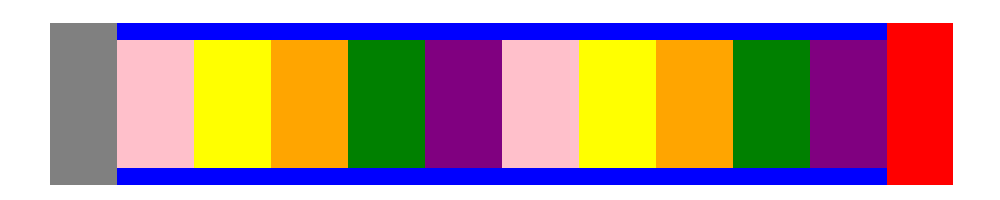
\includegraphics[width=\linewidth]{straightened_slab_mg.png}
    \raggedright
    \resizebox{0.5\textwidth}{!}{
        \hspace{1cm}
        \fbox{\begin{tabular}{llll}
            \textcolor{fhrblue}{$\blacksquare$} & FLiBe & 
            \textcolor{fhrgrey}{$\blacksquare$} & Left Graphite \\
            \textcolor{fhrred}{$\blacksquare$} & Right Graphite &
            \textcolor{fhrpink}{$\blacksquare$} & Fuel cell 1/6 \\
            \textcolor{fhryellow}{$\blacksquare$} & Fuel cell 2/7 &
            \textcolor{fhrorange}{$\blacksquare$} & Fuel cell 3/8 \\
            \textcolor{fhrgreen}{$\blacksquare$} & Fuel cell 4/9 &
            \textcolor{fhrpurple}{$\blacksquare$} & Fuel cell 5/10 \\
            \end{tabular}}}
    \caption{Straightened \acrfull{AHTR} fuel slab spatially discretized into 
    13 \textit{cells} for OpenMC multigroup calculation.}
    \label{fig:straightened_slab_mg}
\end{figure}

For spatial homogenization of the \gls{AHTR} one-third assembly... 
% include details about spatial homogenization for one-third assembly. 

To ensure that the spatial and energy homogenization preserves accuracy, I 
compared key neutronics parameters for the continuous OpenMC and multigroup 
Moltres simulations, for both the \gls{AHTR} plank and one-third assembly.
The results of the verification studies are described in Section 
\ref{sec:ahtr_model_verification}.

\subsection{Output Parameter Calculation}
\label{sec:ahtr_slab_output}
This section describes how I tallied the AHTR model outputs for the ROLLO 
optimization problem objectives (as described in Table \ref{tab:objectives}):
total fuel packing fraction, the maximum temperature in the slab, and 
normalized power peaking factor.  

\gls{ROLLO} will automatically return the total fuel packing fraction output parameter, 
since it is also an input parameter. 
In the Moltres AHTR model, I defined a post processor object to return the 
maximum temperature in the slab. 


\section{AHTR Model Verification}
\label{sec:ahtr_model_verification}

\section{ROLLO Hyperparameter Tuning}